\chapter{Synthèse des activités de recherches} % Main chapter title

\label{synthese} % For referencing the chapter elsewhere, use \ref{Chapter1}

\section{Préabule et déroulement de carrière}
J’ai un parcours scientifique atypique qui s’est construit sur un cursus universitaire alternant formations diplômantes et expériences professionnelles. Mes premiers contacts avec le monde de la recherche scientifique date de 1998. Après une maîtrise de biochimie, j’ai eu l’opportunité de travailler sur des protocoles expérimentaux en biologie moléculaire au sein d’équipes de recherche de l’INRA. En 1999, j’ai poursuivi ces expériences professionnelles au CIRAD pour développer et analyser une banque de marqueurs microsatellites chez le cacao. J’ai pu alors constater l’importance de l’informatique pour la gestion et le traitement des données à l’échelle de la biomolécule. Un tel constat m’a conduit à compléter ma formation de biologiste avec une année de DESS en informatique. J’ai pu alors aborder les problématiques associées à l’organisation et au traitement des données moléculaires sous un angle nouveau lors du stage de fin de cursus du DESS en 2000, qui s’est déroulé dans la même unité de recherche. \\

Mon parcours scientifique a démarré en 2001 suite à l'obtention du cursus universitaire DESS informatique, en tant qu’ingénieur d’étude en bioinformatique (IE2) dans le groupe d’E. Guiderdoni au CIRAD (UMR AGAP) et dans le contexte du projet ANR Génoplante « Analyse fonctionnelle du génome du riz : création d'une collection de 15.000 lignées de mutants d'insertion de riz ».  L'objectif de ce projet était de créer et caractériser une collection de mutants T-DNA chez la variété O. sativa ssp nipponbarre. Le projet était très ambitieux sur le plan informatique et comprenait en effet tous les aspects de traitement de séquences génomiques mais aussi l’informatisation des processus d’analyse phénotypique (qui relèvent de ce que l’on appelle aujourd’hui le phénome). Un défi du projet portait sur la mise en place d’un système intégré, pouvant répondre aux attentes de différentes  équipes de recherche localisées sur différents sites géographiques. Très rapidement mes activités ont concerné des problèmes qui au-delà de la haute technicité impliquaient des réflexions méthodologiques liées à la gestion de données et de connaissances hétérogènes. C’est dans ce contexte que j’ai effectué ma thèse. J’ai bénéficié de l’encadrement  de Thérèse Libourel ( Pr. LIRMM, directeur ), d’Isabelle Mougneot (Mdc LIRMM - Univ. Montpellier) et Manuel Ruiz (Chercheur Cirad). D’un point de vue méthodologique, j’ai défini une structure de médiation (paradigme médiateur/adaptateur) reposant sur un schéma global construit sur l'ensemble des vues sur les schémas sources permettant une consultation unifiée de différentes sources de données hétérogènes dans le contexte de la génomique fonctionnelle. Le médiateur mis en place s’appuyait sur l’approche GAV (Global As View) avec un ensemble de vues sur les schémas des sources de données qui tient lieu de schéma global. J’ai obtenu un poste d’ingénieur d’études CNRS dans l’équipe “Intégration des Données” (ID) dirigée par M. Ruiz au CIRAD (UMR AGAP) quelques temps avant de soutenir ma thèse (cf. schéma \ref{overview}. \\

J’ai poursuivi dans cette voie autour des méthodes d’intégration de données dans le domaine agronomique et je me suis par ailleurs impliqué dans l’animation de la plate-forme bioinformatique SouthGreen.  \\
Je me suis d’abords orienté sur le développement de méthodes automatisant la création d’adaptateurs sémantiques et la formulation de requêtes pour des bases de données biologiques en co-encadrant la thèse de Julien Wollbrett (voir section \ref{SWS}).\\

Par la suite, j’ai quitté le CNRS en 2010, pour effectuer une mobilité au sein de l’IRD dans l’équipe Génome et Développement du Riz (UMR DIADE) dont les enjeux en matière de partage et d’intégration de données génomiques étaient particulièrement motivants. Je me suis également fortement impliqué dans la structuration d’une plateforme bioinformatique naissante transversale sur plusieurs unités IRD. \\
Afin de répondre aux besoins de gestion des masses de données produites par le séquencage et le phénotypage de nouvelles variétés de riz, j’ai développé des méthodes d’intégration et de stockage basées sur des architectures distribuées détaillées en section \ref{GIGWA}. \\
Entre 2012 et 2017, j'ai été impliqué dans le projet « Institut de Biologie Computationnelle » (IBC). IBC est un projet ANR « investissement d’avenir » en bioinformatique dont l’objectif était de développer de nouvelles méthodes et logiciels pour le traitement des grandes masses de données biologiques avec des applications dans les domaines de la santé, l’agronomie et l’environnement. 
Jusqu'en 2017, j'ai été co-responsable de l’axe « intégration des données et connaissances biologiques » qui reprenait les problématiques d’intégration de données pour la biologie des plantes. Je me suis fortement impliqué dans cette tâche car les problématiques sont très importantes pour l’unité DIADE. Pour mener à bien cette coordination, j’ai partagé mon temps entre les locaux d’IBC situé au LIRMM et l’équipe RICE. J’ai pu ainsi créer une synergie entre experts de différents domaines de l’informatique et de la biologie afin d’avancer sur des points tels que la gestion des données phénomiques et la gestion des données NGS (Next Generation Sequencing). Mes activités de recherches menées dans le cadre du projet IBC sont décrites en section \ref{IBC}. \\
Depuis le mois de septembre 2016, je travaille mandaté par l'IRD en expatriation au Vietnam pour développer in situ des approches bioinformatiques avec les partenaires Vietnamiens du LMI RICE\footnote{\url{https://sites.google.com/site/lmiricevn}}, afin de permettre une meilleure exploitation de leurs données. Récemment fin 2017, j’ai pris la responsabilité du laboratoire informatique IRD-USTH (Université des Sciences et Techniques d’Hanoi). Le laboratoire compte neuf jeunes enseignants chercheurs en informatique avec qui je collabore sur certains aspects méthodologiques. Par ailleurs, je consacre une partie de mon temps à l’enseignement en Masters (Informatique et Biologie) ainsi qu’à l’encadrement d’étudiants. Je développe également des collaborations avec l’ International Rice Research Institute (IRRI) qui est un des centres du Consultative Group on International Agricultural Research (CGIAR) sur le Riz basé aux Philippines.
J'ai récemment obtenu un poste de chargé de recherche à l'IRD en présentant les thématiques que je décris dans ce mémoire. \\

\begin{figure}[!ht]
\begin{center}
	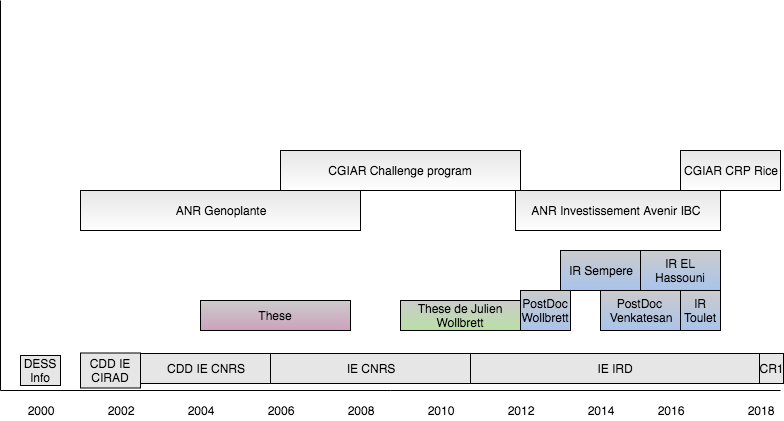
\includegraphics[width=1\textwidth]{Figures/Parcours-overview.png}
\end{center}
\caption{\label{overview} Schéma de mon parcours recherche}
\end{figure}



\section{Activités de recherche en cours}

Les progrès de la génomique et des outils de phénotypage à haut débit offrent une occasion unique de découvrir de nouveaux gènes. Les ressources génétiques peuvent maintenant être séquencées à faible coût pour étudier de manière fine leur diversité génétique. Les systèmes d'information actuels permettent de plus en plus l'intégration de données hétérogènes, cependant de nombreux challenges existent encore lorsqu'ils s'agit d'exploiter le croisement de ces données d'autant plus que ces données sont massives et multi-échelles. De nombreux challenges résident dans le traitement de l'information sous-jacente afin de découvrir rapidement des relations gène-phénotype et leur dépendance à l’environnement qui détermine le rendement des cultures dans des environnements divers.

\subsection*{Mise en place d’approches pour l’interopérabilité des bases de données biologiques}\label{these}

Dans le contexte du projet ANR Genoplante, une collection de mutant T-DNA de riz a été crée puis caractérisée dans l'objectif d'étudier les fonctions de la totalité des gènes de riz. Son étude comprenait le séquençage des gènes mutés par le T-DNA (et d'autres éléments génomiques mobiles) ainsi que la caractérisation phénotypique des lignées de mutants sur plusieurs sites géographiques. J'ai eu la charge du volet bio-informatique. J'ai ainsi développé un workflow de détection et d'annotation des  gènes disruptés par le T-DNA nommés ``Flanquing Sequence Tag'' (FST)  (2004-02). J'ai également été impliqué, dans le développement de l'application OrygenesDB \footnote{\url{http://orygenesdb.cirad.fr}}, une application web permettant de stocker des données relatives aux séquences générées lors du projet et également les séquences issues du séquençage du génome du riz (2006-01). Le principal objectif de mon travail a été la conception du système d'information dédié à la gestion des données phénotypiques et leur enrichissement par des liens avec les autres ressources (génomique, transcriptomique, protéomique) décrivant la collection. Pour ce faire, j’ai développé OryzaTagLine \footnote{\url{http://oryzatagline.cirad.fr}}, un système d’information permettant d’intégrer et centraliser ces différentes ressources afin de fournir un portail web unique aux scientifiques (2008-01).\\

Au cours de ce projet, je me suis engagé sur une thèse afin de lever de nombreux verrous liés à l’intégration de données dans le domaine agronomique. Les thématiques abordées concernaient (i) la formalisation de standards d’échange de données, de métadonnées et d’ontologies pour décrire et annoter les données, (ii) le développement d’infrastructures permettant la communication d’applications sur des réseaux distribués. L’objectif de mon travail était de permettre aux scientifiques d'accéder de manière transparente aux informations issues de plusieurs sources de données (génomique, phénotypique, etc.).  Pour cela, j’ai abordé le sujet en développant deux approches : une architecture de médiation et une architecture orienté services (SOA).  

\paragraph*{Adaptation de Le Select pour la médiation de ressources végétales} La première approche proposait l'intégration de sources à travers l'adaptation d'un système de médiation de données : Le Select~\cite{manolescu2002}. Successeur de DISCO~\cite{Tomasic1998}, Le Select utilisait un modèle pivot relationnel proche du SQL, afin d’intégrer de manière transparente les sources de données hétérogènes et distribuées. Le fait que Le Select utilise le standard SQL, lui permettait d’interagir avec un bon nombre d’applications s’appuyant sur ce standard.
Les données ont une représentation uniforme exprimée dans le modèle de données relationnel étendu à des types de données définis par l'utilisateur (e.g. structurés, semi-structurés, etc). Ecrit en Java, le médiateur propose également un accès uniforme à l’exécution de programmes intégrés (e.g. services, programmes) ainsi que la publication et le traitement des données issues de ces processus. De manière générale, Le Select offrait des outils de transformation des données publiées et permettait d’attacher une documentation structurée sur ces dernières. D’un point de vue réseau, Le Select avait une architecture distribuée de type mediateur/adaptateur, ce qui veut dire qu’il n’existait pas de dépot centralisé pour intégrer les données, ni de schéma global. En effet plusieurs applications Le Select peuvaient coopérer pour fournir l’accès aux ressources. Publier par exemple, des systèmes d’information par l’intermédiaire de Le Select évitait de mettre à jour les données intégrées et maintient leur autonomie vis à vis d’autres applications clientes. Ces avantages, nous voulions les mettre à profit dans le cadre d’un projet scientifique visant l’intégration de ressources de données végétales (2006-02). 

Dans un premier temps, mes travaux ont consisté à l'intégration syntactique de plusieurs sources de données à l'aide de Le Select par la mise en place d'adaptateurs. Plusieurs sources étaient identifiées dont celles du CIRAD (incluant Orya Tag Line et OrygenesDB), une à l'IRD, une au CNRS (Univ. Perpignan) et une banque d'image au CIAT (Colombie). Dans de nombreux cas, il s'agissait d'instancier des librairies génériques proposées par le médiateur (base de données, fichiers structurés, exécution de programmes, etc.). Par la suite, des métadonnées ont été générées et associées aux adaptateurs. Par exemple, des métadonnées ont été extraites automatiquement des systèmes de fichiers et des images pour instancier les adaptateurs de la banque d'image. Ces métadonnées étaient importantes pour que les médiateurs communiquant en réseau, identifient les sources intervenant dans une requête de médiateur ,

Concernant l'intégration sémantique, Le Select ne proposait pas de mécanisme particulier pour détecter des correspondances (mappings) entre les éléments des sources. Seul des mécanismes de vues (identiques à ceux des bases de données relationnelles) pouvaient etre utilisés à cette fin.  Ainsi, des règles ACI (correspondance inter-schéma) ont été développées pour chaque adaptateur au niveau des tables et des attributs. La traduction des éléments en ACI a été réalisée selon des règles établies par le document de spécification ODM  \footnote{\url{https://www.omg.org/spec/ODM/About-ODM}}. Un schéma global sous la forme d'une vue a été construit sur la base des schémas exposés par les adaptateurs des instances Le Select. Les règles ACI ont été prise en compte dans la construction. Finalement,  une ontologie en OWL DL a été développée sur la base du schéma global dans l'objectif de support au mapping pour l'intégration de nouvelles sources.  Enfin, afin de montrer l'intéret d'une infrastructure de médiation distribuée dans ce contexte, une mise en oeuvre de l'intégration sémantique a été illustrée à travers des exemples de recherche d'information biologique. \\

\paragraph*{Intégration de données par le biais de Service Web} La deuxième approche proposait l’intégration des sources à travers l’enchaînement de services web (SW) grâce à un environnement web personnalisé (2008-02). Ce système utilisait le Framework BioMoby~\cite{Wilkinson2002a,Wilkinson2005a}  et son annuaire de services web bioinformatiques utilisant le protocole SOAP. BioMoby est un projet open source essentiellement orienté sur la découverte et l’exécution de SW biologiques. En effet par le biais d’un annuaire central, l’application propose aux fournisseurs d’enregistrer et de décrire leurs services en tenant compte d’un vocabulaire structuré. L’utilisation d’un tel vocabulaire pour décrire les SW permet de faciliter la recherche et l’enchainement des services. Toutefois BioMoby ne propose pas d’outils permettant de gérer les conflits (de noms, lors de l'enregistrement des services. Par ailleurs, il ne propose pas non plus d'outils d’enchainements de SW intégrés à son API. \\
Etant donné que BioMoby était tres utilisé dans la communauté bioinformatique, la gestion des enregistrements de services et l'orchestration de services étaient deux verrous importants. Mes premiers travaux ont porté sur la réalisation d'un système d'enchainement de services BioMoby (2007-01 et 2008-02). Les méthodes développées ont permis d'exposer les systèmes d'information développés au cours me ma thèse (i.e. Oryza Tag Line et OrygenesDB) avec des Services Web BioMoby. Des méthodes ont été développées pour orchestrer ces SW avec d'autres services BioMoby. Ces méthodes comprenaient des composants permettant de déterminer i) le type de données (ou d'objet) utilisé par le service, ii) rechercher les services compatibles, iii) determiner les étapes pouvant etre exécutées en parralèle,  iv) serialiser les résultats dans divers formats. Par ailleurs, une application web a été développée afin de permettre l'utilisation de ces méthodes par un public de biologistes. \\

Mes contributions développées au cours de ma thèse, ont permis de généraliser l’utilisation des standards d’échanges de données (au sein du CIRAD et de ses partenaires) ainsi que d’appliquer différentes approches d’intégration de données en agronomie. Elles ont également permis d’accroitre les fonctionnalités des applications OryzaTagLine et OrygenesDB et leur interopérabilité avec d’autres systèmes existants.

% expliquer SOAP
\subsubsection*{Sélection de références}

\begin{itemize}

\item (2004-02) Sallaud C., Gay C., Larmande P., Bès M., Piffanelli P., Piégu B., Droc G., Regad F., Bourgeois E., Meynard D., Périn C., Sabau X., Ghesquière A., Delseny M., Glaszmann J.C., Guiderdoni, E. (2004) High throughput T-DNA insertion mutagenesis in rice : A first step towards in silico reverse genetics. Plant J. 2004 Aug; 39(3):450-64. Impact Factor: 5.468      
\item (2006-01) Droc G, Ruiz M, Larmande P, Pereira A, Piffanelli P, Morel JB, Dievart A, Courtois B, Guiderdoni E, Périn C. OryGenesDB: a database for rice reverse genetics. Nucleic Acids Res. 2006 Jan 1; 34(Database issue):D736-40. Impact factor: 9.202
\item (2006-02) Pierre Larmande, Christine Tranchant-Dubreuil, L. Regnier, Isabelle Mougenot, Thérèse Libourel:
Integration of Data Sources for Plant Genomics. ICEIS (1) 2006: 314-318
\item (2007-01) Pierre Larmande. A personalized integrated system for rice functional genomic. 2007, Poster, NETTAB, Pise, Italie.
\item (2008-01) Larmande P, Gay C, Lorieux M, Périn C, Bouniol M, Droc G, Sallaud C, Perez P, Barnola I, Biderre-Petit C, Martin J, Morel JB, Johnson AA, Bourgis F, Ghesquière, A, Ruiz M, Courtois B, Guiderdoni E. Oryza Tag Line, a phenotypic mutant database for the Genoplante rice insertion line library. Nucleic Acids Res. 2008 Jan; 36(Database issue):D1022-7. Impact factor: 9.202 
\item (2008-02) Droc G, Périn C, Fromentin S, Larmande P. OryGenesDB 2008 update: database interoperability for functional genomics of rice. Nucleic Acids Res. 2009 Jan; 37 (Database issue):D992-5. Impact factor: 9.202

\end{itemize}

\subsection*{Génération automatique de services web pour les bases de données relationnelles biologiques}
\label{SWS}

Ayant rejoint l’équipe intégration des données de M. Ruiz, j’ai été impliqué dans le projet international Generation Challenge Programme (GCP), l’un des cinq Challenge Programme établis par le Consultative Group on International Agricultural of Research (CGIAR).  \\

Une plateforme d’intégration de données, nommée GCP Pantheon, avait été développée afin de permettre à des clients logiciels d’interroger de manière transparente tout type de données générées dans le cadre du programme GCP. Cette plateforme combinait une approche de médiation LAV (Local As View) et une approche sémantique, permettant aux partenaires de gérer leurs données localement puis de les rendre accessibles facilement en accord avec un modèle conçu spécifiquement pour le projet, GCP Domain Model~\cite{Bruskiewich2006,Bruskiewich2008}. Le modèle GCP a également été utilisé pour implémenter le Framework BioMoby qui s’était rapidement imposé comme protocole standard d’échanges de données et de services dans le domaine bioinformatique.\\

La principale limitation de la plateforme GCP Pantheon était due au « mapping » manuel des schémas des sources locales sur le schéma global du GCP Domain Model. Afin de lever cette limitation, j’ai co-encadré une thèse (thèse de Julien Wollbrett) sur les méthodes de création automatique d’adaptateurs, facilitant ainsi l’intégration sémantique des bases de données relationnelles biologiques sur la GCP. A cet effet, la thèse exploitait l’utilisation de différentes ontologies de domaines (génomique, phénotypiques, etc.) permettant l’établissement à la fois des règles de correspondance et d’interprétation, nécessaires à l’intégration automatisée. 

Le point commun de l’intégration de données et des technologies du Web Sémantique est de dépasser l’hétérogénéité sémantique de sources de données interconnectées. Le Web Sémantique facilite la représentation de la sémantique des données et peut ainsi être utilisé pour faciliter l’interopérabilité ou l’intégration de données~\cite{antezana2009,Jonquet2010}. Parmi les technologies utilisées pour exposer des données sur le Web de données RDF, RDFS, OWL et SPARQL sont les éléments importants.\\

\textbf{RDF (Resource Description Framework)} est largement utilisé pour intégrer des données issues de plusieurs sources. Ceci est dû au cadre qu'il fournit pour décrire une ressource et ses relations sous la forme de triplets, Subject-Predicate-Object. Ces triplets peuvent être combinés pour construire un grand réseau d'informations (également connu sous le nom de graphe RDF), intégré à partir de différentes sources de données. %## Peut être bien expliquer que parmi les standards du web semantique on trouve RDF qui est très souvent utilisé pour formaliser les données et ensuite dire que D2RQ est une plateforme qui permet d'accéder aux SGBD relationnels via une vision RDF. ##

L'intégration de base de données relationnelles (BDR) en utilisant les standards du Web Sémantique est confrontée à une problématique de mise en correspondance (mapping) entre des schémas de BDR et une ou plusieurs ontologies. De nombreuses approches de mapping entre BDR et RDF ont été proposées ces dernières années afin de répondre à plusieurs motivations. La production de logiciels implémentant ces diverses approches fut toutefois marquée le logiciel D2RQ~\cite{Bizer2003,Bizer2004} et par la spécification récente d’un langage de mapping nommé R2RML~\cite{Souripriya} dont la recommendation est apparue après nos travaux. Nous renvoyons les lecteurs vers une synthèse exhaustive des approches et outils de mapping~\cite{Antipolis2014}.\\

Peu d’outils disponibles au début du projet (2010) utilisaient des standards du web sémantique, que ce soit pour la vue du schéma de la BDR (RDF, XML), ou pour le langage de requête (SPARQL), et permettaient de mapper une base de données avec plus d’une ontologie. Considérant les outils Virtuoso et D2RQ dans notre approche, nous avons choisi d'utiliser D2RQ. Il s'agit d'une plateforme de publication de BDR sur le Web utilisant les standards du Web Sémantique et permettant de traiter une base de données relationnelle comme un graphe virtuel RDF. Dans ce graphe un élément du schéma est représenté par un nœud et une relation par un arc orienté. Il est possible de créer ce graphe virtuel RDF en exportant uniquement le schéma de la BDR et donc aucune instance. Nous parlerons alors de vue RDF. La plateforme D2RQ est composée de 3 éléments principaux. i) Le langage déclaratif de mapping D2RQ, utilisé pour créer la vue RDF de la BDR et permettant de décrire les relations entre des ontologies et un schéma de BDR. ii) Le moteur D2RQ permettant de créer automatiquement une vue RDF et de transformer une requête SPARQL interrogeant la vue RDF en une requête SQL interrogeant directement la BDR. iii) le Serveur HTTP D2R permettant d’interroger les bases de données relationnelles via le Web.\\

Dans notre approche nous avons décidé de détourner D2RQ pour, en plus d'homogénéiser des schémas hétérogènes, automatiser la création de requêtes sur des BDR distribuées. Pour cela nous avons enrichi sémantiquement et de manière automatique la vue RDF du schéma de BDR créée par D2RQ. Nous avons ensuite travaillé sur la formulation de requêtes se basant sur les vues RDF ainsi générées en développant un algorithme de recherche de plus court chemin dans les graphes RDF~\cite{wollbrett2013clever} capable de prendre en compte les particularités des schémas relationnels. Nous avons ainsi, développé BioSemantic, une approche flexible, générique et automatisée en nous appuyant sur des standards du Web Sémantique et des Services Web (2013-01). \\

BioSemantic propose la création d'adaptateurs en 2 étapes distinctes. Une première étape consiste à créer automatiquement une vue RDF du schéma de la BDR à intégrer, puis à annoter manuellement cette vue à l'aide de termes ontologiques. L'étape d'annotation est la seule nécessitant un utilisateur expert ayant une connaissance du schéma de la BDR à intégrer. La 2ème étape est l'étape de création d'adaptateurs à proprement parler. Elle utilise toutes les vues RDF précédemment créées et annotées pour créer automatiquement des adaptateurs. Dans cette seconde étape aucune connaissance des schémas de BDR n'est nécessaire. La seule nécessité est la connaissance des termes ontologiques utilisés dans le schéma global. La création de ces adaptateurs est basée à la fois sur un enrichissement sémantique de la vue RDF créée par D2RQ et sur la notion de parcours de graphe.\\

L'utilisation de D2RQ dans BioSemantic présente plusieurs avantages comme la présence d'un langage déclaratif permettant de définir des mappings complexes entre le schéma de la BDR et des termes ontologiques. Un autre avantage est la présence du moteur D2RQ permettant de transformer automatiquement une requête SPARQL interrogeant une vue RDF en une requête SQL interrogeant la BDR sans exporter ses données. De plus, l'utilisation de RDF et son formalisme en triplet va nous permettre de parcourir la vue RDF comme un graphe et ainsi virtuellement parcourir le schéma de la BDR pour trouver une requête pertinente à intégrer dans notre adaptateur. Nous allons donc utiliser D2RQ tout en détournant son utilisation pour automatiser la création de requêtes SPARQL.

\paragraph*{Limites de l'utilisation de D2RQ dans BioSemantic}
Nous souhaitons utiliser le langage D2RQ pour parcourir notre vue RDF et ainsi indirectement parcourir notre schéma de BDR. D2RQ n'ayant pas été implémenté pour cette utilisation, le langage D2RQ n'est pas suffisamment expressif pour définir toutes les relations que nous souhaiterions. Il permet par exemple de définir des clés primaires et des clés étrangères mais ne permet pas de définir une table d'association ou d'autres spécificités à prendre en compte pour notre parcours de la vue RDF dans le but de créer automatiquement une requête pertinente. Une requête créée automatiquement sera considérée comme pertinente si les données qu'elle renvoie sont identiques aux données renvoyées par une requête créée manuellement par un expert du schéma de la BDR.

\subsubsection*{Enrichissement sémantique d'une vue RDF D2RQ}
\paragraph*{La combinaison de chemins}
Lors de la création de requête, il faut tenir compte du contexte spécifique de la recherche de plus court chemin dans un schéma de base de données relationnelle. Une des spécificités de notre schéma relationnel par rapport à un simple graphe, est la présence de relations bien définies entre les tables. Notre recherche de plus court chemin doit donc tenir compte des spécificités de ces relations.\\

Les relations concernées sont :\\
\begin{itemize}
\item \textbf{La relation d'agrégation}: par défaut, une association exprime une relation à couplage faible. Les entités associées restent relativement indépendantes l'une de l'autre [11]. L'agrégation est une forme particulière d'association qui exprime un couplage plus fort entre entités. Elle permet d'exprimer des relations de type maître/esclaves et représente des connexions bidirectionnelles dissymétriques. \\
\item \textbf{La relation de composition}: il s'agit d'une forme d'agrégation avec couplage plus important entre les entités. Cette composition indique que la destruction de l'agrégat entraîne automatiquement la destruction des composants agrégés.\\
\item \textbf{La relation d'héritage}: la généralisation et la spécialisation sont des points de vue portés sur les hiérarchies d'entités. Une entité A est une spécialisation d'une entité B si chaque instance de A est une instance de B et si chaque instance de B est associée à au plus une instance de A.\\

\end{itemize}

Nous nous sommes intéressés aux relations d'agrégation et d'héritage car elles présentent une particularité commune susceptible de nous intéresser. Toutes les entités spécialisées, issues d'une même relation d'héritage, sont indépendantes. Cela signifie que l'intersection des instances qu'elle contient est vide. Cette propriété est également présente dans les entités agrégées issues d'un même agrégat et pourrait être utilisé pour combiner différents chemins pour créer notre requête sans que cette dernière ne renvoie des données redondantes.  Cela peut poser des problèmes si on souhaite créer automatiquement une requête en utilisant un algorithme de recherche de plus court chemin, seul le chemin ayant le moins de nœuds intermédiaires serait détecté.
%Nous allons illustrer l'intérêt de la combinaison de chemins à l'aide de l'exemple présent dans le schéma d'entité-association de la Figure \ref{heritage}. Dans ce schéma on peut voir une relation d'héritage. Les entités Etude\_de\_genotypage et Etude\_de\_phenotypage sont des spécialisations d'une Etude. Une étude est donc soit une étude de génotypage, soit une étude de phénotypage. Cela peut poser des problèmes si on souhaite créer automatiquement une requête qui, pour un identifiant d'étude donné, renvoie tous les noms de germplasme associés. En utilisant un algorithme de recherche de plus court chemin, seul le chemin ayant le moins de nœuds intermédiaires permettant de relier Etude à Germplasme serait détecté. Ce chemin serait utilisé pour créer une requête composée de jointure entre ces tables. Cela signifie que si un identifiant donné correspond à un identifiant d'Etude\_de\_genotypage, la requête créée automatiquement ne renverra aucune donnée. 
Dans le cas de relations d'héritage dans un schéma entité-association, il faut donc utiliser une combinaison de chemins pour la création de requêtes. Cependant, pour savoir comment prendre en compte ce type de relation, il faut s'intéresser aux règles de conversion de ce type de relation du modèle entité-association au modèle relationnel.

%\begin{figure}[!ht]
%\begin{center}
%	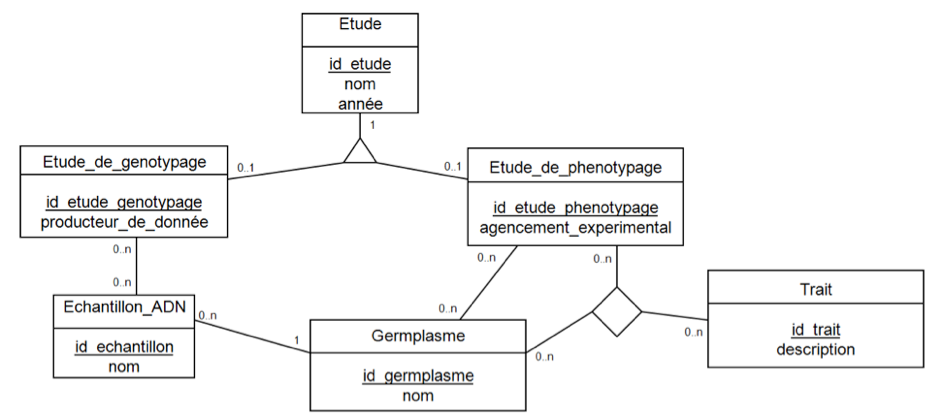
\includegraphics[width=1\textwidth]{Figures/biosemantic1.png}
%\end{center}
%\caption{\label{heritage} Schéma entité-association montrant une relation d'héritage.}
%\end{figure}

\paragraph*{Passage au modèle relationnel}

La conversion d'une relation d'héritage peut s'effectuer de trois façons différentes lors du passage du modèle entité-association vers le modèle relationnel [12] aplati vers le haut, aplati vers le bas ou non aplati. Les relations d'héritage aplaties vers le haut et vers le bas ne posent pas de problème de combinaison de chemin lors de notre recherche de plus court chemin. En suivant une approche non aplatie, chaque entité est convertie en une relation.  Une clé étrangère supplémentaire, correspondant à la clé primaire de la relation généraliste, est présente dans chaque relation spécialisée. 

%Le modèle résultant est le suivant:

%\begin{verbatimtab}
%etude(id_etude, nom, annee)
%	echantillon_ADN(id_echantillon, nom, #id_germplasme)
%	germplasme(id_germplasme, nom)
%	etude_de_genotypage (id_etude_genotypage, 
%		producteur_de_donnee, #id_etude)
%	etude_de_phenotypage(id_etude_phenotypage, 
%		agencement_experimental, #id_etude)
%	echantillon_genotypage (#id_echantillon,#id_etude_genotypage)
%	germplasme_phenotypage (#id_germplasme, #id_etude_phenotypage)
%\end{verbatimtab}
%
%Ici les attributs soulignés correspondent à des clés primaires et les attributs précédés d'un dièse correspondent à des clés étrangères. Lors d'une conversion vers une relation d'héritage non aplati, les relations spécialisées et généralistes sont présentes physiquement. Cela signifie qu'une relation est créée pour chaque entité. Dans ces conditions, la création d'une requête prenant en entrée la relation généraliste peut nécessiter de combiner plusieurs chemins. Pour la conversion non aplatie de la relation d'héritage, présentée dans notre exemple, la création d'une requête renvoyant tous les Germplasmes pour une étude donnée nécessitera la combinaison des plus courts chemins passant par les relations Etude\_de\_genotypage et Etude\_de\_phenotypage.

\paragraph*{Détection des relations d'héritage non aplaties}

La détection automatique de relations d'héritage non aplati pour la transformation d’un schéma relationnel vers une ontologie a été décrite dans [13]. Elle est également utilisée pour typer les relations d'héritage de l’outil DB2OWL [14]. Cette détection automatique est basée sur les techniques de retroconception dans les BDR, tentant notamment de convertir un modèle relationnel en modèle entité association [15]. Cette détection utilise la particularité des contraintes d'intégrité entre les tables généralistes et les tables spécialisées. En effet, pour qu'une table soit une spécialisation d'une autre table, elle doit contenir pour seule clé étrangère la clé primaire de la table généraliste. Dans un article plus récent, les auteurs démontrent que ce type de transformation n’est possible dans le cas ou les BDR respectent la troisième forme normale [16]. La détection automatique de ce genre de relation d'héritage est alors rendue possible en utilisant la règle suivante:

\begin{verbatimtab}
Subclass(r,s) <- Rel(r)^Rel(s)^PK(x,r)^FK(x,r,_,s)
avec
Rel(r)	r est une relation
PK(x,r)	x est la clé primaire de r
FK(x,r,y,s) x est la clé primaire de la relation r 
	et référence y dans la relations
\end{verbatimtab}

L'utilisation de cette règle rend automatique la détection de toutes les relations d'héritage non aplaties. Elle détecte également les relations d'agrégation ou de composition, nous permettant donc de détecter tous les types de chemins que nous souhaitions combiner lors de la création de nos requêtes.

\paragraph*{Enrichissement de la vue RDF}
Nous avons décidé d'ajouter cette information directement dans la vue RDF, à l'aide de la propriété rdfs:SubClassOf issue du vocabulaire RDF. Dans notre cas, la détection de relation d'héritage implique la création de deux nouveaux triplets dans la vue RDF comme dans l'exemple ci-dessous correspondant au schéma \ref{graph}. 

\begin{verbatimtab}
etude_de_genotypage 	rdfs:subClassOf 	etude
etude_de_phenotypage	rdfs:subClassOf 	etude
\end{verbatimtab}

\subsubsection*{Prise en compte de la pondération dans la sélection de chemin}
La simple prise en compte du nombre de nœuds à parcourir pour déterminer la longueur du plus court chemin ne prend pas en compte la diversité d'associations présentes dans un schéma relationnel. Dans notre vue RDF nous n'avons pas accès aux cardinalités des associations. Nous ne pouvons donc pas utiliser ce critère pour favoriser le passage par une association plutôt que par une autre. Nous avons par contre accès aux clés primaires et clés étrangères. Nous allons donc utiliser ces paramètres pour tenter d'optimiser l'algorithme de détection de plus court chemin. Nous allons dans un premier temps nous intéresser aux tables d'associations puis aux arités des relations. Le passage par des tables d'association d'arité supérieure à 2 peut induire une perte d'information. Nous avons donc intérêt à favoriser le passage par les tables d'association binaires mais également de pénaliser le passage par les tables d'association d'arité supérieure à 2.

\paragraph*{Détection des tables d'association et de leur arité}
La Figure \ref{algo} présente l'algorithme de détection des tables d'association avec attributs.


\begin{figure}[!ht]
\begin{center}
	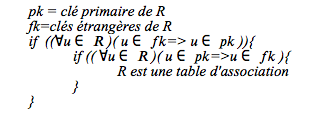
\includegraphics[width=0.7\textwidth]{Figures/algo-arite.png}
\end{center}
\caption{\label{algo} Algorithme de détection des tables d'association avec attributs.}
\end{figure}

Une table d'association sans attributs est un cas particulier de table d'association. Il s'agit d'une table associant 2 autres tables et dont les seules colonnes sont celles correspondant aux clés primaires des 2 tables associées. Ce type de table d'association est typé comme une propriété dans la vue RDF D2RQ. La détection de ces tables d'association sans attributs se fait automatiquement en détectant les propriétés de la vue RDF possédant plusieurs clés étrangères. Dans la vue RDF, l'information sur l'arité d'une table d'association est transcrite indirectement. Cette arité peut être trouvée automatiquement en détectant le nombre de clés étrangères présentent dans une table d'association.

\paragraph*{Enrichissement de la vue RDF D2RQ}
Les tables d'associations possédant ou non des attributs sont annotées avec la propriété \textit{dr:associatedTo}. Un triplet contenant ce prédicat sera ajouté pour chaque table associée. Le sujet de ce triplet correspondra à la table d'association et l'objet à la table associée. L’arité d’une table d’association est annotée avec la propriété \textit{dr:arity}. Ce typage est réalisé automatiquement, sous la forme de triplets, lors de la création de la vue RDF.

\subsubsection*{Utilisation de l'enrichissement dans la recherche de plus court chemin}
Ce schéma a conduit à la création d'une vue RDF dont la représentation sous forme de graphe est présentée dans la Figure \ref{graph}. Dans ce graphe, seul les nœuds représentant des tables sont présents, ces nœuds sont de couleur orange. Les nœuds rouges représentent les annotations sémantiques, ajoutées manuellement, réalisées sur une colonne de la table associée. Les arcs noirs représentent des propriétés présentes d’origine dans la vue RDF, et les arcs rouges représentent les arcs rajoutés automatiquement par notre approche. Les nœuds bleus représentent la valeur associée à l’arité d’une table d’association, qui est détectée automatiquement. Pour créer une requête SPARQL, nous utilisons les annotations sémantiques ajoutées manuellement dans la vue RDF d'un schéma de BDR. Dans l’exemple de la Figure 5, nous allons sélectionner les annotations sémantiques \textit{gcpdm:etude} et \textit{gcpdm:germplasm} pour créer automatiquement une requête renvoyant tous les germplasms d'une étude donnée. 

\begin{figure}[!ht]
\begin{center}
	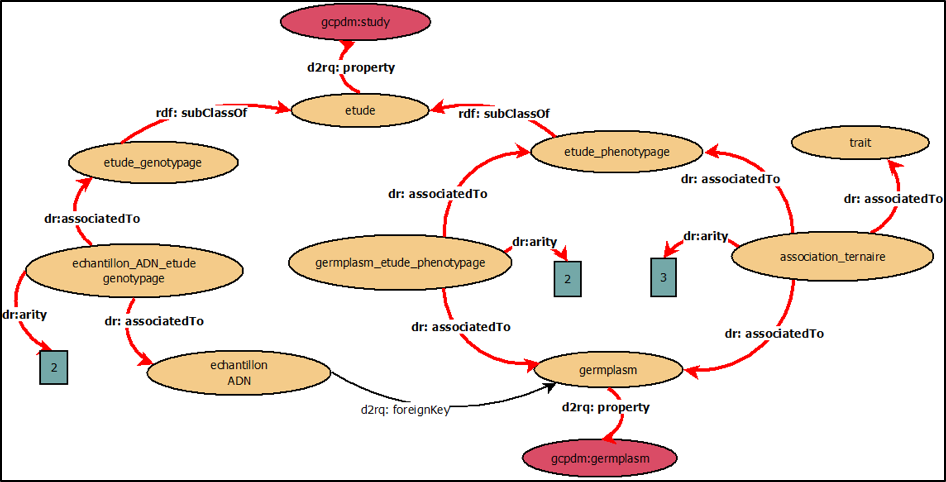
\includegraphics[width=1\textwidth]{Figures/biosemantic3.png}
\end{center}
\caption{\label{graph} Graphe représentant la vue RDF du schéma de la base de données utilisée comme exemple de la création de requête SPARQL.}
\end{figure}

Lors de la recherche de plus court chemin, l'algorithme va détecter une relation de spécialisation entre la table etude et les tables etude\_genotypage et etude\_phenotypage grâce à l'enrichissement sémantique avec les balises rdf:subclassOf. Cette information va être prise en compte et le plus court chemin renvoyé sera donc l'agrégation des plus courts chemins passant par ces 2 tables spécialisées (flèches rouges de l'étape A de la Figure \ref{parcours}). Lors du passage par la table etude\_phenotypage, l'algorithme a la possibilité de trouver 2 chemins passant par le même nombre de noeuds. Le premier chemin passe par la table d'association binaire germplasm\_etude\_phenotypage et le deuxième chemin par la table d'association ternaire appelée ici asociation\_ternaire. L'enrichissement sémantique avec les balises dr:associatedTo permet à l'algorithme de détecter l'arité de ces tables d'association et de choisir de passer par celle ayant l'arité la plus petite. Dans l'exemple de l'étape B de la Figure \ref{parcours}, l'algorithme passera par la flèche rouge de gauche et ne parcourra pas la portion de graphe passant par la flèche rouge droite. Le plus court chemin final renvoyé par notre algorithme, permettant de créer automatiquement une requête pertinente, est représenté dans l'étape C de la Figure \ref{parcours}.


\begin{figure}[!ht]
\begin{center}
	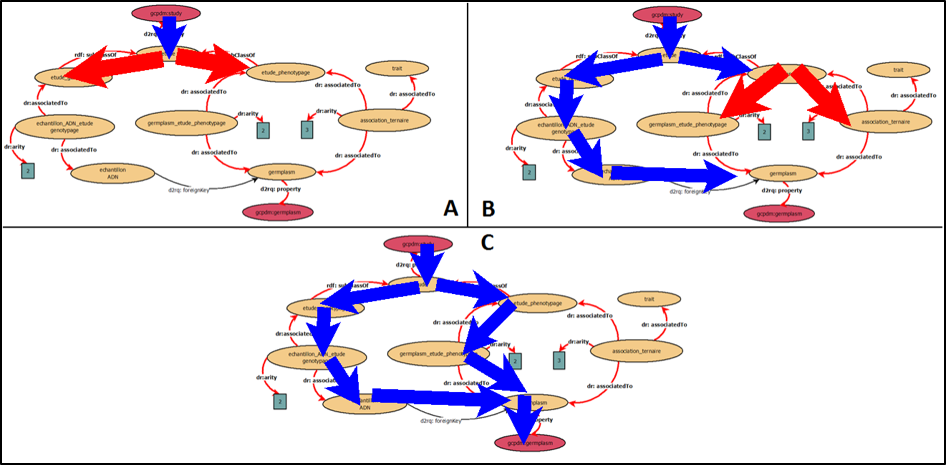
\includegraphics[width=1\textwidth]{Figures/biosemantic4.png}
\end{center}
\caption{\label{parcours} Utilisation de l'enrichissement sémantique dans le parcours de graphe.}
\end{figure}

\subsubsection*{Sélection de références}

\begin{itemize}

\item (2013-01) Wollbrett J, Larmande P, De Lamotte F, Ruiz M. Clever creation of rich SPARQL queries from annotated relational schema: application to Semantic Web Service creation. BMC Bioinformatics. 2013. Impact Factor: 2.435
\end{itemize}

\subsection*{Passage à l’échelle dans l’analyse des variations génomiques}
\label{GIGWA}

Les enjeux du stockage et traitement des données génomiques sont au cœur des problématiques de l’unité DIADE IRD. L’équipe RICE coordonne le projet IRIGIN (International RIce Genomic Initiative) dont l’objectif est de réaliser le re-séquençage de centaines de variétés de riz et le génotypage par séquençage de milliers de lignées de riz, avec l’équivalent de 18 000 génomes de riz en termes de volume de données (90 TeraBytes). Aujourd'hui bien que les biologistes ont souvent encore l'habitude de manipuler leurs données à l'aide de logiciels de type tableur, les données devenant massives et complexes leurs en limite l'utilisation. Il en resulte que les alternatives souvent proposées passent par l’utilisation de logiciels exécutables lignes de commande dans un environnement Unix.
Depuis 2013, je coordonne le développement d’un logiciel nommée Gigwa qui facilite cette tâche. Gigwa est une application qui utilise la technologie de base de données NoSQL (MongoDB) afin de gérer le passage à l’échelle pour le stockage et l’analyse des données de variations génomiques (typiquement issus de fichiers VCF, standard de représentation des variants génomiques), et d’offrir une interface WEB permettant d’y appliquer des filtres. Ce système permet alors de naviguer dans les résultats et de ré-exporter ces sous-jeux de données sous divers formats standardisés et de visualiser les variations dans leur contexte génomique. La contribution novatrice dans ce projet réside dans le modèle de stockage de données, que nous avons défini et optimisé pour ce type de données. De plus, le modèle tire avantage de la flexibilité d’extension du SGBD et permet d’utiliser l’application sur un ordinateur de bureau comme sur un cluster de calcul en distribuant les données sur plusieurs nœuds. Bien entendu, les performances tiennent compte du volume de données stockées et des ressources allouées, mais nous obtenons des résultats encourageant par rapport aux autres applications leader dans ce domaine. Un article effectuant le comparatif et décrivant l'application a été publié en 2016 (2016-01).
% updater avec les resultats du nouvel article
% ajouter un paragraphe sur le bechmark 

Actuellement, nous développons une API de services REST pour Gigwa comme alternative à son interface web. Cette API qui respecte et étend les recommandations du GA4GH Data Working Group\footnote{\url{http://ga4gh.org}} et de la Breeding API\footnote{\url{https://brapi.org}} permettra d’accroitre l’interopérabilité de l’application avec d’autres systèmes utilisés dans la communauté bioinformatique tels que Galaxy~\cite{Giardine2005,Goecks2010}, FlapJack~\cite{Milne2010}, SniPlay~\cite{Dereeper2015} ou Toggle~\cite{Monat2015}.

\paragraph*{De la masse de données à la connaissance}
En perspective d’extraire de la connaissance dans cette masse d’information génomique, nous avons commencé à explorer les possibilités que peuvent offrir les approches de « mapping » entre le web sémantique et les bases de données NoSQL orientées documents (e.g., MongoDB). Dans le cadre du projet spirale IRD BIOeSAI, un système d’information a été développé pour stocker des expérimentations en utilisant MongoDB (2015-01). Ces expérimentations requièrent la manipulation d’un volume important de données qui de fait sont de nature hétérogènes et stockées sous des formes différentes (fichier Excel, texte structuré ou semi-structure, images, etc.). Ce volume et cette diversité de données peuvent rendre leur exploitation par les chercheurs difficile et non optimale. Dans ce contexte, un systeme d’intégration et d'indexation générique a été développé afin de pouvoir naviguer, partager et annoter ces données dans le but de les exploiter au mieux. L'aspect novateur de ce projet réside dans la mise au point d'un système évolutif permettant aux utilisateurs d’effectuer toutes les étapes allant de l’intégration de données jusqu’a la composition de requêtes. Ce système inclut également la gestion des métadonnées et des annotations ajoutés par les utilisateurs. Toutefois, la méthode mise en place ne permet pas de détecter des relations explicites/implicites entre les données gérées par le système.  Par exemple, il n’est pas possible de déduire qu’une région géographique (localisation GPS ou décrite) est inclue dans une region plus large afin d’agréger des résultats. Ou encore, il est impossible de propager une information qui est implicite comme une maladie affectant toute la plante affectera tous ses tissus. \\
Au cours de son stage de M2, Luyen Le Ngoc évalua plusieurs approches pour mapper le schéma du système (Document JSON) à un modèle RDF annoté avec des ontologies biologiques~\cite{Luyen:2016} (2016-02). Il aborda notamment les approches de matérialisation de données en triplets RDF avec xR2RML~\cite{Michel2015} et de ré-écriture de requêtes avec les applications Ontop~\cite{rodriguez}, xR2RML et AllegroGraph. Puis dans une autre optique de materialisation, il évalua l'application NEO4J à partir d'import de données JSON. Enfin, il évalua également, l'utilisation de MongoDB avec des documents JSON-LD comme source de stochage et Jena pour la gestion des triplets RDF. \\

La solution retenue fut l'approche xR2RML avec une matérialisation en RDF pour des bases de petites tailles et une ré-écriture pour des bases plus importantes. Toutefois, cette dernière approche n'a pas été évaluée faute de temps. 

Afin de répondre à la question de passage à l'échelle pour la gestion de triplets RDF, nous avons également évalué plusieurs triple-stores: Sesame, 4Store, Virtuoso, Jena Fuseki, StarDog, AllegroGraph et GraphDB.  L'évaluation porta sur différents critères à savoir:
\begin{itemize}
\item le chargement de données; 
\item la recherche d'information avec projection, filtre, tri, union;
\item la recherche d'information avec plusieurs type d'inférences.\\
\end{itemize}


Une architecture présentée en figure \ref{mongo}, a été développée afin de tester les différentes opérations sur les triplestores. Une couche médiatrice logicielle orchestrait les différentes tâches à tester. Les tests ont été réalisés sur des données réelles produites par le projet Phenome et stockées dans la base de données PHIS (INRA)~\cite{neveu2018}. Elles comportaient à la fois des données textuelles et des images avec méta-données associées.  Une ontologie développée par l'équipe de Pascal Neveu (Phis) a été utilisée pour effectuer des requêtes d'inférences sur les données triplifiées.


\begin{figure}[!ht]
\begin{center}
	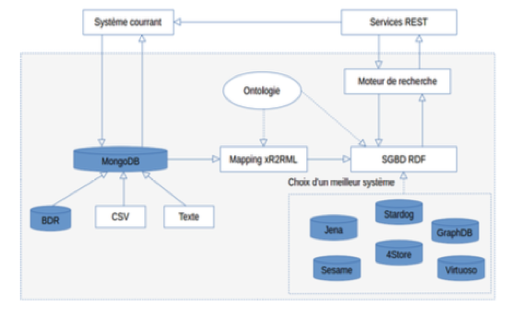
\includegraphics[width=1\textwidth]{Figures/MongoRDF.png}
\end{center}
\caption{\label{mongo} Architecture de l'application réalisée pour mettre en place le benchmark.}
\end{figure}
Parmi les solutions commerciales, StarDog a obenu de trés bon résultats sur l'ensemble des tests. Virtuoso édition libre, a obtenu de bons résultats pour les logiciels libres. Ces résultats nous ont confortés dans l'utilisation de Virtuoso pour la suite de nos travaux.

\subsubsection*{Sélection de références}

\begin{itemize}
\item (2016-01) Sempéré G, Philippe F, Dereeper A, Ruiz M, Sarah G, Larmande P. Gigwa—Genotype investigator for genome- wide analyses. Gigascience. 2016. 5:25. Impact Factor : 7.463
\item (2016-02) Le Ngoc L, Tireau A, Venkatesan A, Neveu P, Larmande P. Development of a knowledge system for Big Data: Case study to phenotyping data. Int. Conf. Web Intell. Min. Semant. Proceedings ACM WIMS ’16. 2016. Nimes (France)
\item (2015-01) Le Ngoc L., Jouannic S. and Larmande P. Développement d'un outil générique d'indexation pour optimiser l'exploitation de données biologiques. Poster aux Journées ouvertes pour la Biologie, l’informatique et les Mathematiques JOBIM 2015. Clermont-Ferrant (France)
\end{itemize}


\subsection*{Intégration sémantique des données agronomiques}
\label{IBC}

Entre 2013 et 2017, j'ai été impliqué dans le projet « Institut de Biologie Computationnelle » (IBC) et ai été coordinateur de l’axe « intégration des données et connaissances biologiques » qui reprenait les problématiques d’intégration de données pour la biologie des plantes.

Nous avons dans un premier temps, contribué au développement de méthodes automatiques d’intégration de bases de données biologiques en associant les logiciels WebSmatch~\cite{Coletta2012}, développé par l’équipe INRIA Zénith, Bioportal~\cite{Noy2009,Melzi} et Biosemantic~\cite{wollbrett2013clever} en réalisant un prototype~\cite{castanier2014semantic}. Ce travail a permis d’identifier un besoin dans l’annotation sémantique des données et la gestion des ontologies pour le domaine des plantes. \\

\paragraph*{La plateforme AgroPortal} Avec Clément Jonquet (MdC Lirmm), nous avons réalisé un premier prototype d’entrepôt d’ontologie nommé AgroPortal. Le projet Agroportal vise à développer un portail d'ontologies de référence pour le domaine de l'agronomie. Une première version de la plateforme est d’ores et déjà déployée et maintenue sur un serveur du LIRMM \footnote{\url{http://agroportal.lirmm.fr}}. 

La plateforme AgroPortal~\cite{Jonquet2016,Jonquet2018} reprend la technologie du NCBO BioPortal (portail pour la santé et les ontologies biomédicales, \footnote{\url{http://bioportal.bioontology.org}}. Cette technologie est open-source et indépendante du domaine thématique concerné. Le portail propose des services de recherche d'ontologie et de visualisation, avec la possibilité de déposer des commentaires et des notes. Il offre également un service d'annotation sémantique de données avec les ontologies. L'objectif principal de ce projet est de permettre une utilisation simple des ontologies liées au domaine de l'agronomie, en proposant aux chercheurs de prendre en charge les questions d'ingénierie des connaissances complexes pour annoter les données de recherche. De nombreuses contributions scientifiques ont été réalisées pour améliorer les fonctionnalités du portail. Des nouvelles méthodes de scores~\cite{Melzi} ont été développées pour classer les mappings avec des termes ontologiques. Un nouvel algorithme de recommandation a été implémenté dans le \textit{Recommender}~\cite{RomeroJOGPM16} et un nouveau modèle de métadonnées a été développé et implémenté dans la plateforme~\cite{toulet:lirmm-01397388}.\\

\paragraph*{La plateforme AgroLD} Ainsi, une infrastructure capaple de gérer des ontologies du domaine agronomique et de proposer des services pour rechercher, annoter les données, etc. etait dorénavant disponible. Toutefois, les données ainsi annotées sémantiquement nécessitaient une infrastructure permettant de les gérer efficacement. Or, il existait des projets équivalents dans le domaine biomédical et bioinformatique Bio2RDF~\cite{Belleau2008a,Callahan2013}, EBI RDF~\cite{Jupp2014}, ou encore Uniprot RDF~\cite{redaschi2009}  mais pas encore de projet dans le domaine agronomique. Avec l’aide d’un post-doctorant recruté dans le projet IBC en 2014, nous avons élaboré des modèles de données et développé un premier prototype de système d’intégration sémantique de ressources biologiques (AgroLD\footnote{\url{http://www.agrold.org}}). AgroLD est une base de connaissance utilisant les technologies du web sémantique comme structure pour intégrer les données. AgroLD est conçue pour intégrer des informations disponibles sur diverses espèces végétales du domaine agronomique telles que les espèces de riz (Oryza), Arabidopsis, le blé et le sorgho. Le cadre conceptuel de la connaissance est basé sur des ontologies bien établies dans le domaine telles que Gene Ontology ~\cite{Ashburner2000,TheGeneOntologyConsortium2014}, Plant Ontology~\cite{plantOntology2002}, Plant Trait Ontology~\cite{planteome2018}, Plant Environement Ontology~\cite{envo2016} pour n'en citer que quelques unes dont la majorité sont hébergées par le projet OBO Foundry~\cite{Smith2007}. En outre, compte tenu de la portée de l'effort, nous avons décidé de construire AgroLD en plusieurs phases. La phase actuelle (phase un) couvre les informations sur les gènes, les protéines, les prédictions de gènes homologues, les voies métaboliques, des phénotypes de plantes et le matériel génétique. A ce stade nous avons intégré des données issues plusieurs ressources telles que Gramene~\cite{gramene2018} , UniProtKB~\cite{uniprot2011} , Gene Ontology Annotation~\cite{goa2009}  ainsi que des ressources développées par la plateforme SouthGreen\footnote{\url{http://southgreen.fr/}} comme TropGeneDB~\cite{tropgenedb2012}, OryGenesDB~\cite{Droc2009b} , GreenPhylDB~\cite{greenphyl2011} , OryzaTagLine~\cite{larmande2008} , SniPlay~\cite{sniplay3}.  Le tableau \ref{sources} donne un appercu des espèces et sources intégrées. Entre 2015 et 2017, l’institut Français de bioinformatique (IFB) a financé notre projet à travers le projet IFB plant node   “Développement d’un réseau de ressources bioinformatiques sémantiquement interconnectées” (coord. M. Ruiz) permettant ainsi d'étendre l'intégration sur un nombre d'espèces plus important.


\begin{landscape}
\begin{center}
\begin{table}[h]
\begin{tabular}{|p{3 cm}| p{6 cm}|p{2 cm}|p{2 cm}| p{3 cm}|p{3 cm}|p{2 cm}|} 
\hline
 \textbf{Sources de données} & \textbf{URLs} & \textbf{Format de fichier} & \textbf{Nb Tuples} & \textbf{Especes} & \textbf{Ontologies utilisées} & \textbf{Nb de triplets produits} \\
 \hline
 Oryzabase & shigen.nig.ac.jp/& Custom flat file & 17K  & R & GO,PO,TO & 153K \\ 
 GO associations & geneontology.org & GAF &1, 160K & R, W, A, M, S & GO & 2, 700K \\ 
 OryGenesDB & orygenesdb.cirad.fr & GFF & 1, 100K&R, S, A, & GO, SO & 2, 300K \\ 
 Gramene & gramene.org & Custom flat file & 1, 718K & R, W, M, A, S & GO, PO, TO, EO & 5, 172K \\ 
 UniprotKB & uniprot.org & Custom flat file & 1, 400K & R, W, A, M, S & GO, PO & 50, 000 K \\ 
 Oryza Tag Line & oryzatagline.cirad.fr & Custom flat file & 22K & R & PO, TO, CO & 300K \\ 
 TropGeneDB & tropgenedb.cirad.fr & Custom flat file & 2K & R & PO, TO, CO & 20K \\ 
 GreenPhylDB & greenphyl.org & Custom flat file & 100K & R,A & GO, PO  & 700K \\ 
 SNiPlay & sniplay.southgreen.fr & HapMap, VCF & 16K & R & GO  & 16,000K \\ 
 Q-TARO & Qtaro.abr.affrc.go.jp & Custom flat file & 2K & R & PO, TO  & 20K \\ 
 \textbf{TOTAL} &  & &  & &   & \textbf{87,400K} \\ 
 \hline
\end{tabular}
\newline
\caption{\label{sources} \textbf{Les espèces et les sources de données intégrées dans AgroLD.} Le nombre de tuples donne une idée du nombre d’éléments que nous avons ont annoté à partir des sources de données (par exemple, 1, 160K Gene Ontology annotations). Especes et Ontologies sont référencées suivant R = riz, W = blé, A = Arabidopsis, S = sorgho, M = maïs, GO = gene ontology, PO = plant ontology, TO = plant trait ontology, EO =  plant environnment  ontology, SO =  sequence ontology, CO = crop ontology (caracteres spécifiques des plantes).
134 ontologies)}
\end{table}
\end{center}
\end{landscape}


Nos contributions portent sur la création de différents workflows de transformation RDF pour des grands jeux de données agronomiques. Même si de nombreux outils étaient disponibles au sein de la communauté du Web Sémantique, parmi eux citons datalift\footnote{\url{https://project.inria.fr/datalift}} ou csv2rdf4lod\footnote{\url{http://purl.org/twc/id/software/csv2rdf4lod}}, aucun n'étaient adaptés pour prendre en compte la complexité des formats de fichiers plats du domaine biologique ou même la complexite des informations qu'ils peuvaint contenir. Déjà, initié avec le projet BioSemantic, nous avons étendus ces modèles de transformation à une plus large palette de standards de données en génomique et phénomique tels que le Generic Feature Format (GFF)\footnote{\url{http://gmod.org/wiki/GFF3}}, le Gene Ontology Annotation File\footnote{\url{http://geneontology.org/page/go-annotation-file-format-20}}, le Variant Call Format (VCF)~\cite{danecek2011}, le Genomic Feature and Variation Ontology~\cite{gfvo2015} et le Minimum Information About a Plant Phenotyping Experiment (MIAPPE))~\cite{miappe} et travaillons actuellement à packager ces modèles dans une API \footnote{\url{https://github.com/pierrelarmande/AgroLD-ETL}}. 

Pour cette phase de transformation, chaque jeu de données a été téléchargé à partir de sources sélectionnées et annoté sémantiquement avec des URI de termes ontologiques en réutilisant les identifiants d’ontologie lorsqu’ils ont été fournis par la source d’origine.  À la fin de la phase 1, début 2018, la base de connaissances AgroLD contenait environ 100 millions de triplets RDF créés en convertissant plus de 50 jeux de données provenant de 10 sources de données. De plus, lorsque cela était possible, nous avons utilisé des annotations sémantiques déjà présentes dans les jeux de données, telles que, par exemple, des gènes ou des traits annotés respectivement avec des identifiants GO ou TO (i.e. GO:0005524 est transformé en \url{http://purl.obolibrary.org/obo/GO\_0005524}). Dans ce cas, nous avons généré des propriétés supplémentaires avec les ontologies correspondantes, ajoutant ainsi 22\% de triplets supplémentaires validés manuellement (voir les détails dans le tableau \ref{sources}). Les versions OWL des ontologies candidates ont été directement chargées dans la base de connaissances, mais leurs triplets ne sont pas comptés dans le total.

De plus, nous avons utilisé l'API de service Web AgroPortal pour enrichir les données en annotation sémantiques. Par exemple, pour extraire l'URI correspondant au taxon disponible pour certains standards de données tels que GFF. Mais également pour identifier des concepts ontologiques dans les données comme l'organe d'une plante (e.g. leaf est annoté avec \url{http://purl.obolibrary.org/obo/PO\_0025034}) ou un caractère phénotypique (plant height serait annoté avec le concept ayant pour URI \url{http:// purl.obolibrary. org/obo/TO\_0000207}). Comme le montre la figure \ref{AgroPortal-AgroLD}, le workflow de transformation utilise AgroPortal pour annoter les données au moment de la transformation. De plus, nous avons développé une application spécifique pour traiter les formats de fichiers semi-structurés (tsv, csv, excel)\footnote{\url{https://github.com/pierrelarmande/ontology-project}} et mieux contrôler l'annotation sémantique faite par AgroPortal et y gérer les différentes annotations pour un résultat optimal. 


\begin{figure}[!ht]
\begin{center}
	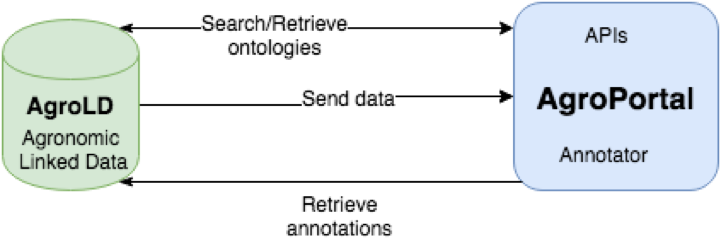
\includegraphics[width=0.90\textwidth]{Figures/AgroPortal-AgroLD.png}
\end{center}
\caption{\label{AgroPortal-AgroLD} Processus d'annotation sémantique entre AgroPortal et AgroLD}
\end{figure}

Les graphes RDF sont nommés d'après les sources de données correspondantes, partageant un espace de noms commun: \url{http://www.southgreen.fr/agrold/}. Les entités dans les graphes RDF sont liées par des URI communs partagés. Comme principe de conception, nous avons utilisé des schémas d'URI mis à disposition par les sources (par exemple, UniprotKB) ou par le registre Identifiers.org~\cite{identifiers}. Par exemple, les protéines de UnitProtKB sont identifiées par l'URI de base: \url{http://purl.uniprot.org/uniprot/}; les gènes intégrés à partir de Gramene / Ensembl plant sont identifiés par l'URI de base: \url{http://identifiers.org/ensembl.plant/}. Lorsqu'elles ne sont pas fournies par les sources ou par Identifiers.org, de nouvelles URI ont été construites tels que TropGene et OryGenesDB; dans ce cas, les URI prennent la forme \url{http://www.southgreen.fr/agrold/[resource\_namespace]/[identifier]}. De plus, les propriétés reliant les entités se présentent sous la forme: \url{http://www.southgreen.fr/agrold/vocabulary/[property]}. À propos de la liaison d'entité, nous avons utilisé «l'approche basée sur la clé» qui est la plus courante. Elle combine l'identifiant unique de l'entité partagée avec la communauté plus le modèle de base d'URI de la ressource. De plus, nous avons également respecté «l’approche URI commune» qui recommande d’utiliser le même modèle d’URI lorsque le même numéro identifiant est utilisé dans différents jeux de données. Par conséquent, définir le même URI pour des entités identiques (représentées par des identificants) dans différents jeux de données permet d'agréger des informations supplémentaires pour cette entité. De plus, nous avons utilisé des liens de références croisées (représentés par des identifiants) en les transformant en URI et en reliant la ressource au prédicat «has\_dbxref». Cela augmente considérablement le nombre de liens sortants, rendant AgroLD plus intégré avec d'autres sources de données. À l'avenir, nous comptons mettre en œuvre une «approche basée sur la similarité» pour identifier les correspondances entre les entités ayant des URI différents (voir deuxieme partie). Enfin, nous avons évalué les différents standards de provenance pouvant être utiliser pour annoter les modèles RDF et les annotations sémantiques (2017-02). 

Afin de faire correspondre les différents types de données et propriétés, nous avons développé un schéma léger\footnote{\url{https://github.com/SouthGreenPlatform/AgroLD}} qui associe les classes et propriétés identifiées dans AgroLD avec des ontologies correspondantes. Par exemple, la classe Protein (\url{http://www.southgreen.fr/agrold/resource/Protein}) est associée à la polypeptide (\url{http://purl.obolibrary.org/obo/SO\_0000104}) de SO avec la propriété \textit{owl: equivalentClass}. Des mappings similaires ont été réalisés pour les propriétés, par exemple, les classes protéines / gènes sont liés aux classes de l'ontologie \textit{molecular function} de GO par la propriété \url{http://www.southgreen.fr/agrold/vocabulary/has\_function}, avec comme propriété \textit{owl: equivalentProperty}. Lorsqu'une propriété équivalente n'existait pas, nous l'avons associé avec la propriété de niveau supérieur avec \textit{rdfs: subPropertyOf}. Par exemple, la propriété \textit{has\_trait} (\url{http://www.southgreen.fr/agrold/vocabulary/has\_trait}), relie les entités aux termes TO équivalent. Elle est associée à une propriété plus générique. Pour l'instant, 55 mappings ont été identifiées. De plus, les mappings sont stockés avec les ontologies dans AgroPortal, ce qui permet des liens directs entre les classes et les instances de ces classes dans AgroLD. Par ailleurs, les classes, les propriétés et les ressources sont déréférencées sur un serveur Pubby~\cite{pubby} dédié (par exemple, \url{http://www.southgreen.fr/agrold/page/biocyc.pathway/CALVIN-PWY}).


En matière d’accès aux graphes de données, même si le langage SPARQL est efficace pour construire les requêtes, il reste difficile à prendre en main pour nos utilisateurs principaux (e.g., bioinformaticiens, biologistes). Ainsi, nous avons proposé un modèle d'architecture implémentant divers éléments constituant de systèmes de recherche sémantique (i.e., formulation de requêtes basé sur des patrons, visualisation sous forme de graphe, outils de recherche d’information) (2017-01).
Ainsi la plateforme AgroLD fournit 4 points d'entrée:\\

\begin{itemize}
\item  \textbf{Quick Search}\footnote{\url{http://www.agrold.org/quicksearch.jsp}}, un plugin de recherche à facettes mis à disposition par Virtuoso, qui permet aux utilisateurs d'effectuer des recherche par mots-clés et de parcourir le contenu d’AgroLD en naviguant dans les liens;\\
\item \textbf{SPARQL Editor}\footnote{\url{http://www.agrold.org/sparqleditor.jsp}}, un éditeur de requêtes SPARQL qui fournit un environnement interactif pour la formulation de requêtes SPARQL. Avec un étudiant de M2, nous avons développé l'éditeur en se basant sur les outils YASQE et YASR~\cite{yasgui} et l'avons adapté pour notre système. Le langage SPARQL est un outil puissant pour extraire des informations utiles de la base de connaissances. Par exemple, sur une requête simple \textit{Identify wheat proteins that are involved in root development (ontology term)} en utilisant Quick Search, renverrait 73 résultats alors qu'utiliser un property path dans une requête SPARQL renverrait 137 résultats. Par ailleurs, le language SPARQL étant plus expréssif il est possible de composer des requêtes complexes recherchant sur plusieurs graphes. Toutefois, parceque SPARQL est difficile à apréhender pour les utilisateurs non-averti, nous avons proposé une liste de patrons de requêtes modulaires et personnalisables en fonction des besoins des utilisateurs qui peuvent être automatiquement exécutées à travers l'éditeur. Accessoirement, des outils fonctionnels ont été ajouté comme la possibilité d'enregister la requête et de télécharger les résultats dans divers formats tels que JSON, TSV et RDF / XML. De plus, les requêtes créées par l'utilisateur peuvent également être chargées dans l'editeur;\\
\item \textbf{Explore Relationships}\footnote{\url{http://www.agrold.org/relfinder.jsp}}, est une implémentation de RelFinder~\cite{relfinder} qui permet aux utilisateurs d’explorer et de visualiser les relations existantes entre entités. Les relations entre des objets constituent une information importante. Ce mode de recherche permet de partir d’un point de départ et explorer le graphe, ou éliminer des parties du graphe des données à l’aide de filtres pour découvrir des relations. Ces techniques présentent malheureusement l’inconvénient de demander beaucoup d’effort manuel de la part de l’utilisateur. L’application RelFinder découvre automatiquement de telles relations dans une source de données disposant d’un serveur d’accès SPARQL et les affiche sous forme de graphe. Elle aide l’utilisateur à trouver les entités avec une fonctionnalité d’auto-complétion associée à une gestion des cas d’ambiguité où les résultats sont classés par ordre de pertinence (entités ayant le plus de label contenant l’expression saisie). Cependant, la version d'origine de RelFinder a été développée (en ActionScript) et configurée pour DBpedia. Nous avons proposé une configuration et une modification du système adapté à AgroLD. La configuration concerne principalement le point d’accès SPARQL, les propriétés à prendre en compte pour la recherche d’entités et la description des ressources. De plus, nous avons ajouté quelques exemples biologiques pour guider les utilisateurs;\\
\item \textbf{Advanced Search}\footnote{\url{http://www.agrold.org/advancedSearch.jsp}}, un formulaire proposant des recherches spécifiques par entité et possédant un moteur d'agrégation de ressources externes. Le formulaire Advanced Search est basé sur une API REST\footnote{\url{http://www.agrold.org/api-doc.jsp}}, entièrement développée dans le cadre du projet AgroLD. Le but de ce formulaire est de fournir aux utilisateurs non-techniques un outil permettant d’interroger la base de connaissances tout en masquant les aspects techniques de la formulation de requêtes SPARQL. L'intérêt de coupler API et formulaire est de pouvoir combiner de manière interactive des recherches dans la base de connaissances et dans des services externes à la fois par l'inteface utilisateur mais également par la programmation.\\

\end{itemize}

Le projet AgroLD nous a permis d’identifier de nombreux challenges sur le plan informatique ouvrant de nouvelles pistes de travail. \\
\textbf{Dans le domaine de la Recherche d’Information} nous avons commencé à travailler sur l’indexation des graphes RDF et leur enrichissement sémantique (2016-04). Afin d'améliorer la fonctionnalité Quick Search en récupérant plus d'informations textuelles et en masquant les détails techniques, nous avons développé un outil d'indexation permettant de communiquer facilement entre Virtuoso et des clusters Elastic. Ainsi, cet outil permet d’indexer les fichiers Json et de gérer les index (par exemple, mettre à jour, supprimer) sur des clusters Elastic sans utiliser cURL. La difficulté résidait dans le passage d'une structure de donnée sous forme de graphe dans un document document JSON où les relations sont par nature applatis. Par exemple, des fonctionnalité de chainage des propriétés ont été développées afin de récuprérer l'infomation textuelles associées aux propritétés des triplets. Par ailleurs, l'indexation des URI et identifiants de bases de données externes ont été rendu plus explicites en utilisant des fonctions de recherche http pour récupérer de l'information supplementaire. De plus, nous avons développé un outil d'annotation générique qui facilite la communication avec NCBO Annotator pour annoter des fichiers JSON avec des ontologies disponibles à partir d'AgroPortal ~\cite{Jonquet2018}. Nous utilisons cet outil avec AgroPortal Annotator pour enrichir et indexer les fichiers Json avec des informations supplémentaires à partir de termes ontologiques tels que des labels, des synonymes, des termes parents et enfants, etc.

Toujours dans l'objectif de réduire la barrière de language pour interroger la base de connaissances, nous avons évaluer des systèmes de question-réponses (SQR) pour la traduction langage naturel en SPARQL. Ce sont des systèmes permettant aux utilisateurs de poser des questions en langage naturel et de leur donner des réponses concises~\cite{HirschmanGaizauskas2001,Lopez-al2011}. Actuellement, les systèmes SQR sont utilisés dans divers domaines et peuvent également être une solution prometteuse pour la biologie végétale. Dans le domaine médical, plusieurs travaux ont été menés qui étaient intéressants d’évaluer, d'exploiter voire d’étendre. Nous avons développé un test de référence (\textit{Gold Standard\footnote{Gold Standard: est le meilleur test du moment permettant d'évaluer une méthode, dans notre cas il s'agissait d'évaluer les méthodes sur des données agronomiques qui étaient absentes des gold standard actuels.}}) afin d'évaluer ces systèmes car les données agronomiques étaient absentes des gold standard actuels (2016-05). Nous avons regroupées différentes informations de la littérature ~\cite{HirschmanGaizauskas2001,Lopez-al2011,Moldovan-al2002,NevesLeser2015} pour mettre en place une classification des systèmes SQR en fonction des principales approches explicitées précédemment, illustrées à la figure \ref{SQR}, et éffectué une évaluation empirique de ces systèmes. Finalement, nous avons porté notre attention sur le système LODQA~\cite{KimCohen2013}. Le système est basé sur 3 modules i) decomposition de la phrase en language naturel, ii) un module de correspondance de termes, iii) réécriture en requête SPARQL. LODQA étant trés dépendant du domaine, dont les mots sont indexés dans le module 2, les tests que nous avons réalisés n'ont pas donnés de bons résultats. Il n'a pas été possible durant le stage de contribuer sur le module de correspondance de termes.

\begin{figure}[!ht]
\begin{center}
	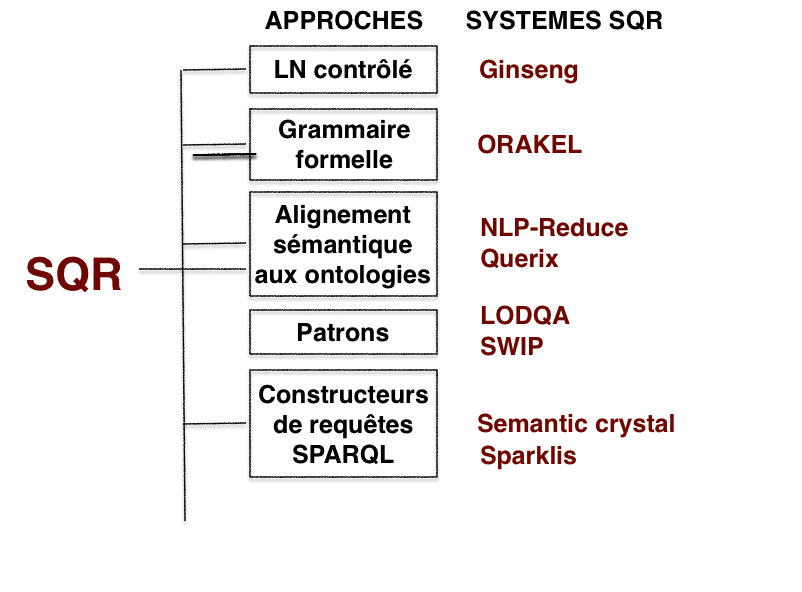
\includegraphics[width=0.90\textwidth]{Figures/classificationSQR.png}
\end{center}
\caption{\label{SQR} Vue générale de notre classification SQR}
\end{figure}

\subsubsection*{Sélection de références} 
\begin{itemize}
\item (2018-0') Do H., Than K., and Larmande P. Evaluating Named-Entity Recognition approaches in plant molecular biology. MIWAI 2018.Proceedings LNCS AI; 2018 (In Press)
\item (2018-03) Larmande P., El Hassouni N. , Venkatesan A., Tagny G., Ruiz M. The Agronomic Linked Data project (AgroLD): a knowledge network platform for rice. Oral presentation at International Symposium on Rice Functional Genomics ISRFG 2017. Sewon (Korea)
\item  (2018-02) Venkatesan A., Tagny G., El Hassouni N., Chentli I., Guignon V., Jonquet C., Ruiz M., and Larmande P. Agronomic Linked Data (AgroLD): a Knowledge\-based System to Enable Integrative Biology in Agronomy. Plos One (In Press) Impact Factor: 2.766
\item (2018-01) Jonquet C.,  Toulet A. , Arnaud E.,  Aubin S. {Dzal{\'{e}} Yeumo} E., Emonet V., Graybeal J., Laporte M. A., Musen M. A. Pesce V. and Larmande P. AgroPortal: A vocabulary and ontology repository for agronomy. Computers and Electronics in Agriculture. 2018;144;126-143 Impact Factor: 2.201
\item (2017-07) Larmande P., El Hassouni N. , Venkatesan A., Tagny G., Ruiz M. The Agronomic Linked Data project (AgroLD): a knowledge network platform for rice. Oral presentation at International Symposium on Rice Functional Genomics ISRFG 2017. Sewon (Korea)
\item (2017-06) Venkatesan A., Tagny G., El Hassouni N., Ruiz M., Larmande P. The Agronomic Linked Data project. Computer demo at Plant and Animal Genomes Conference PAG 2017. San Diego, (USA).
\item (2017-04) Dzale Yeumo E, Alaux M, Arnaud E, Aubin S, Baumann U, Buche P, et al. Developing data interoperability using standards: A wheat community use case. F1000Research. 2017;6:1843.
\item (2017-02) Cohen-Boulakia S, Belhajjame K, Collin O, Chopard J, Froidevaux C, Gaignard A, et al. Scientific workflows for computational reproducibility in the life sciences: Status, challenges and opportunities. Futur. Gener. Comput. Syst. 2017;75. Impact Factor: 2.786
\item (2017-01) Ngompé GT, Venkatesan A, Hassouni N, Ruiz M, Larmande P. AgroLD API Une architecture orientée services pour l’extraction de connaissances dans la base de données liées AgroLD. Lavoisier. 2016. 21:133–58. Impact Factor: 1.046
\item (2016-03) Jonquet C, Toulet A, Arnaud E, Aubin S, Yeumo ED, Emonet V, Graybeal J, Musen MA, Pommier C, Larmande P.  2016.  D202: Reusing the NCBO BioPortal technology for agronomy to build AgroPortal. Oral Presentation at International Conference on Biomedical Ontology and BioCreative ICBO BioCreative 2016. Corvalis (USA)
\item (2016-04) Zevio S., El Hassouni N., Ruiz M. and Larmande P. AgroLD indexing tools with ontological annotations. Poster at Semantic Web for Life Science SWAT4LS 2016. Cambridge (UK)
\item (2016-05) Imène Chentli, Pierre Larmande et Konstantin Todorov. Construction d’un gold standard pour les données agronomiques. IC2016, Montpellier, France.
\item (2016-06) Dagmara Robakowska Hyzorek, Marie Mirouze, Pierre Larmande. Integration and Visualization of Epigenome and Mobilome Data in Crops. Journées ouvertes pour la Biologie, l’informatique et les Mathématiques (JOBIM). Lyon, 2016.
\end{itemize}


\section{Investissements au sein de projets scientifiques}
\begin{itemize}
\item Membre du projet ANR PRCE Data to Knowledge in Agriculture and Biodiversity - D2KAB. 850 K euros. Porteur C. Jonquet.
\item Membre du projet international CGIAR – CRP-RICE. 1,5 M euros pour IRD (2017-2022; Co-resp. WP4.5)
\item Membre du projet postdoc Labex Numev. Lingua 75 K euros. Porteur C. Jonquet
\item Porteur du projet BIOeSAI Spirale IRD 2014-2015 pour le Développement d’une application de gestion de données phénotypique chez le riz. 11 K euros 
\item Porteur du projet postdoc Labex Numev. LandPan TOGGLE. 2015-2016. 50 K euros (coord. P. Larmande \& F. Sabot).

\item Porteur du projet postdoc Labex Numev. AgroPortal: an ontology repository for agronomy. 2015-2016. 50 K euros (coord. P. Larmande \& C. Jonquet).

\item Membre du projet ANR Investissement d’Avenir IBC « Institut de Biologie Computationnelle » Modélisation, traitement et analyse des données à grande échelle en biologie, santé, agronomie et environnement. 2012-2017. 2.842 M euros. (Coord. WP5 P. Larmande \& P. Valduriez)

\item Membre du projet IFB plant node  (Institut Francais de Bioinformatique).  Développement d’un réseau de ressources bioinformatiques sémantiquement interconnectées. (INRA – CIRAD – CNRS – INRIA  - IRD). 2014-2018. 400 K euros.  (coord. M. Ruiz) 

\item Membre du projet ANR Bioadapt Africrop  « Documenting African Crop Domestication » Partenaires IRD, CIRAD (Coord Y. Vigouroux) 2013-2017. 698 K euros
\item Membre du projet EvoRepRice : « Studying the evolution of reproductive development in the Oryza genus for the improvement of modern cultivated rice ». (coord.  S. Jouannic \& M. Kater) 2010-2014.  479 K euros
\item Membre du projet MENERGEP « Methodologies and new resources for genotyping and phenotyping of African rice species and their pathogens for developing strategic disease resistance breeding programs». Partners: IRD (DIADE), CIRAD (BGPI), Africarice (A. Ghesquière Coord.) projet CGIAR GRISP 800 K\$ US
\end{itemize}

\section{Responsabilité d'animation de la recherche}

\subsection*{Responsabilité d’équipe}
\subsubsection*{Co-Direction ICT Lab USTH - Hanoi} 
Depuis 2017, suite au depart d’Alexis Drogoul à la repésentation IRD Vietnam, j’ai pris la co-direction du laboratoire mixte IRD-USTH ICT Lab\footnote{\url{http://ictlab.usth.edu.vn}} . Il est composé de 11 chercheurs et enseignants chercheurs. Mon rôle comprend en particulier l’animation scientifique, la gestion du budget, les rapports d’activité, la communication. Cela implique au delà l'idée de développer le projet de recherche en m'appuyant sur les collaborations au sein du laboratoire.

\subsubsection*{Co-responsable du WP5 de l’Institut de Biologie Computationnelle - IBC} 
Entre mi-2013 et debut 2017, j’ai été coordinateur de l’axe wp5 « intégration des données et connaissances biologiques » d'IBC\footnote{\url{http://www.ibc-montpellier.fr}}. L’objectif de cet axe est de faciliter l’accès aux données et connaissances en biologie. Il est composé de 10 chercheurs et ingénieurs collaborant sur plusieurs projets. Mon rôle de coordination comprenait en particulier le suivi des avancements et des livrables, la gestion du budget, les rapports d’activité, la communication. J’y ai également développé de nouvelles méthodes d’intégration sur des données réelles. De plus, j’ai supervisé le travail d’un post doctorant, d’un ingénieur et de stagiaires afin de travailler sur les différents livrables.  


\subsubsection*{Co-responsable du plateau bioinformatique \textit{i-Trop} IRD} 
Le plateau  \textit{i-Trop}\footnote{\url{http://bioinfo.mpl.ird.fr}} est une infrastructure de calcul et de services mise en place et maintenue par le centre IRD de Montpellier pour les unités locales et les partenaires du sud. Les missions de ce plateau sont (i) de proposer un environnement de travail doté de capacité de calcul et de stockage adapté aux besoins des scientifiques, (ii) de centraliser les ressources bioinformatiques nécessaires pour les utilisateurs du plateau. Depuis janvier 2010, j’ai participé au montage et l’animation de cette structure, dont j’ai été le coordinateur en 2012-2013. Je suis actuellement contributeur en termes de services et applications.


\subsection*{Responsable et Membre de Comités d’Organisation}

\subsubsection*{Semantic Web for Biodiversity (S4BIODIV) 2013 } 
S4BIODIV\footnote{\url{http://semantic-biodiversity.mpl.ird.fr}} est un workshop attaché à la conférence ESWC2013. J'ai Co-organisé le workshop avec E.Arnaud, C. Jonquet, T. Libourel, I. Mougenot, M. Ruiz. Montpellier, France.  Proceedings disponibles sur CEUR\footnote{\url{http://ceur-ws.org/Vol-979/}}

\subsubsection*{PhenoHarmonis : Harmonization, semantic and interoperability of phenotypic and agronomic data Workshop 2014 - 2016 - 2018} Suite au succés du workshop S4BIODIV, le groupe d'organisation a travaillé sur cette nouvelle série.  J'ai co-organisé PhenoHarmonIS\footnote{\url{https://tinyurl.com/PhenoharmonIS2018}} avec E. Arnaud, M. Ruiz, P. Neveu, C. Pommier, D. Pot, JF Rami. Montpellier, France.


\subsubsection*{IC2016 : 27e Journées francophones d'Ingénierie des Connaissances  2016 } 6-10 juin. Montpellier, France.  J'ai pu co-organiser la conference en recherchant des financements permettant d'inviter des keynotes speakers. 
 \footnote{\url{https://ic2016.sciencesconf.org}}

\subsubsection*{AgroHackathon: discovering AgroPortal \& AgroLD. 2016 } Premier Hackathon\footnote{\url{https://www.meetup.com/AgroHackathon}} dédié à l’intégration de données agronomiques. Co-organisation avec C. Jonquet. Montpellier, France.


\subsubsection*{RDA Rice Data Interoperability Working Group} Research Data Alliance est une organisation internationale dont l'objectif est de promouvoir les standards d’échange et la publication des données dans la communauté scientifique. Je coordonne depuis janvier 2017, le groupe pour le riz. l'objectif Rice Data Interoperability WG\footnote{\url{https://www.rd-alliance.org/groups/rice-data-interoperability-wg.html}} sera de proposer l’utilisation de standards et un guide de bonnes pratiques pour échanger et publier les données produites sur le riz. 


% mettre du plus ancien au plus recent
\section{Activités d’enseignement}
\begin{itemize}
\item Enseignement de Bioinformatique au Master 2 ICT USTH, \& Bio, 2017-2018 (50h)
\item Enseignement au Master 2 ICT USTH, Systèmes d’information Geographique, 2017 (25h)
\item Enseignement au DESS de Bioinformatique, UMII, TP BioPerl, 2002-2003 (50h)
\item Enseignement IUT Informatique, UMII, TP Base de données, 2004-2006 (120h)
\item Enseignement Master BioPharma USTH (Hanoi), Module Bioinformatique 2013 (40h)
\end{itemize}


\section{Encadrements}

\subsection*{Thèses}

\subsubsection*{2009-2011 J. Wollbrett}
\textit{Title:} Génération semi-automatique de services Web sémantiques pour des bases de données relationnelles biologiques

\begin{itemize}
\item Thèse de l’Université Montpellier II
\item Taux d’encadrement : 50\% avec M.Ruiz et I. Mougenot
\item Soutenance : Dec. 2011
\item Situation actuelle : Post-Doctorant au Swiss Institute of Bioinformatics. Auparavant Post-doctorant au CNRS Roscoff.
\item Financement : Bourse Région LR-CIRAD

\end{itemize}


\subsection*{Stages Post-doctoraux}
% mettre du plus ancien au plus recent

J’ai collaboré avec 3 docteurs en stages post-doctoraux et 2 ingénieurs de recherche.
\begin{description}
\item [+] [2015 – 2017] N. El Hassouni – Contribution dans le développement du projet AgroLD. Financement INRA sur le projet IFB 
\item [+] [2015 - 2017] A. Toulet – Contribution au développement d’un portail d’ontologies pour l’agronomie basé : AgroPortal. Financement Numev puis IBC
o	Co-supervision avec Clément Jonquet
\item [+] [2014 –2016] G. Sempéré – Conception et développement de l’application Gigwa. Financement Cirad.
\item [+] [2014 - 2016] : A. Venkatesan – Intégation de données utilisant les métadonnees et ontologies pour pour agréger les données de plusieurs ressources hétérogenes. Financement IBC
\item [+] [2012-2013] J.Wollbrett - Automatiser l’intégration de bases de données relationnelles distribuées à travers l’enrichissement sémantique de vues RDF avec BioSemantic – Financement Cirad - IBC
\end{description}

\subsection*{Masters }

J’ai encadré 17 masters.
\subsubsection*{Encadrement de stages de master professionnel}
%Annee en gras
\begin{itemize}
\item 2001 C. Tranchant – Développement d’un système d’information sur la traçabilité des échantillons OGM . DESS IAO UMII \\
Situation suivante : Ingénieur Bioinformatique, IRD

\item 2002 G. Droc – Développement d’un pipeline de traitement des séquences génomiques pour les mutants d’insertion chez le riz – Master2 Bioinformatique UMII\\
situation suivante : Ingénieur Bioinformatique, Cirad

\item 2014 F. Philippe -  Analyse de données de variations génétique dans les riz – Master2 bioinformatique Lumini \\
co-encadrement : G. Sempere – Cirad \\
Situation suivante : Ingénieur Bioinformatique, INRA

\item 2017 B. Vautrin – Développement de module ETL pour l’intégration de ressources dans AgroLD. PolyTech. (stage international - Hanoi) \\
Situation suivante : Dernière année polytech 

\item 2017 J-C Idjellidaine – Propososition d’un systeme de recommandation pour valider les mappings sémantiques dans AgroLD. L3 informatique \\
co-encadrement : N. El Hassouni \\
Situation suivante : M1 AIGLE 

\item 2016 A. Petel – Contribution au développement de Gigwa – Master2 Polytech Grenoble \\
co-encadrement : G. Sempéré \\
Situation suivante : Volontaire International Cirad, la Reunion

\item 2016 D. Hyżorek - Epigenetic Data Integration and Analysis – Master2 parcours BCD UM \\
co-encadrement : M. Mirouze \\
Situation suivante : Chercheur en Pologne
\end{itemize}


%annee en gras
% a actualiser

\subsubsection*{Encadrement de stages de master recherche}

\begin{itemize}
\item 2007 S. Fromentin - Développement d’un Framework de services web pour l’interopérabilité de ressources agronomiques - Master2 Bioinformatique Orsay\\
Situation suivante : Consultant Bioinformatique SS2I

\item 2008 J. Wollbrett - Intégration automatique d’une ontologie de domaine dans un annuaire de service web bioinformatique : Biomoby – Master2 Bioinformatique UMII\\
co-encadrement : M. Ruiz – Cirad\\
Situation suivante : Thèse CIRAD-Région LR

\item 2014 G. Tagny (M1) - Développement d’une base de connaissance sur les gènes régulateurs de la ramification chez le riz – Master1 Institut Francophone d’Informatique – Hanoi \\
Situation suivante : Master 2

\item 2014 L. Le Ngoc (M1) - Développement d’une application de gestion de données phénotypique chez le riz – Master1 Institut Francophone d’Informatique – Hanoi \\
Situation suivante : Master 2

\item 2015 I. Chentli - Facilitation de l'accès aux données biologiques sémantiquement structurées – Master2 parcours BCD UM \\
co-encadrement : K. Todorov \\
Situation suivante : Ingénieur Bioinformatique, IMGT-CNRS

\item 2015 L. Le Ngoc (M2) - Développement d’un système connaissances pour BIG DATA : application aux données de phénotypage chez le riz (O. sativa) – Master2 Institut Francophone d’Informatique – Hanoi \\
Co-encadrement: 	Pascal Neveu – INRA \\
Situation suivante : Thèse CIFRE Crédit Agricole, Brest

\item 2015 G. Tagny (M2) - The Agronomic Linked Data (AgroLD) project. Master2 Institut Francophone d’Informatique – Hanoi \\
Co-encadrement : A. Venkatesan \\
Situation suivante : Thèse Ecole des Mines Ales, Nîmes

\item 2016 S. Remini - Acquisition automatique de connaissances à partir de textes scientifiques – Master2 parcours BCD UM \\
co-encadrement : K. Todorov \\ 
Situation suivante : Recherche d’emploi

\item  2016 S. Zevio - Indexation de données issues du web sémantique dans le domaine agronomique – Master1 parcours DECOL UM \\
Situation suivante : Master 2 DECOL UM 

\item  2017 A. Diouf –  Proposition et implémentation d’algorithmes de liage de données RDF dans AgroLD – M1 BCD \\
co-encadrement : K. Todorov \\
Situation suivante : M2 BCD

\item  2018 A. Sayadi –  Liage de données complementaires dans le contexte d'AgroLD – M2 AIGLE \\
co-encadrement : K. Todorov \\
Situation suivante : Recherche d'emploi

\item  2018 H. Do –  Evaluating Name-Entity Recognition approaches in plant molecular biology – M1 USTH \\
co-encadrement : K. Tanh \\
Situation suivante : M2 USTH

\item  2018 K.M. Djibril –  Ontology Matching tool using AgroPortal API – M2 USTH \\
Situation suivante : Job
\end{itemize}

\section{Autres implications}
\subsection*{Relectures d’articles}
\begin{itemize}
\item Nucleic Acids Research, 
\item Databases, 
\item BMC Bioinformatics, 
\item Current Plant Biology
\end{itemize}

\subsection*{JURYS}
\begin{itemize}
\item Rapporteur de stages de M2 Bio-Informatique (UM) (régulièrement depuis 2002)
\item Jury Masters BioPharma USTH 2017
\item Jury de concours CNRS (Ingénieur d’Etude)
\end{itemize}

\subsection*{Expertises}
\begin{itemize}
\item Membre extérieur de comité d’évaluation des agents CIRAD
\item Membre de comité d'évaluation des départements Bio et ICT USTH
\end{itemize}


\section{Prototypage}
\begin{itemize}
\item  AgroLD\footnote{\url{http://www.agrold.org}} – Visualisation des données sous forme de graphes RDF, constructeur de requêtes, API de services web.
% 
\item GIGWA\footnote{\url{http://gigwa.southgreen.fr}}  – Développement d’une base de données génomiques, constructeur de requêtes, API de services web. Co-encadrement G. Sempere.
% 
\item BIOeSAI\footnote{\url{http://vmbioesai-dev.ird.fr:8080/Syspherice}} - Développement d’une base de données phénotypique, constructeur de requêtes 
\item BioSemantic\footnote{\url{http://www.southgreen.fr/content/biosemantic-tool}} - Développement d’un constructeur de requêtes SPARQL au-dessus de bases de données relationnelles biologiques. Co-encadrement M. Ruiz
%
\item OryGenesDB\footnote{\url{ http://orygenesdb.cirad.fr}} - Développement d’une base de données génomique pour le riz.
\item Oryza Tag line\footnote{\url{http://oryzatagline.cirad.fr}} - Développement d’une base de données de mutant phénotypiques pour le riz.  
\item Détection de motifs « FST » dans les séquences nucléiques du genome Oryza Sativa (Riz)
\end{itemize}
%